\documentclass[nouppercase]{ifmbe}

\title{Robust CSP and LDA for BCI Applications}

\affiliation{Institution/Department, Affiliation, City, Country}{FIRSTAFF}

\author{A.B. Firstauthor1}{FIRSTAFF}
\author{C. Coauthor2}{FIRSTAFF}
\author{D.E. Othercoauthor1}{FIRSTAFF}

%\affiliation{Instituto Tecnol\'{o}gico de Buenos Aires/Computer Engineering Department, Buenos Aires, Argentina }{FIRSTAFF}

%\author{R.Ramele}{FIRSTAFF}
%\author{A.J.Villar}{FIRSTAFF}
%\author{J.M.Santos}{FIRSTAFF}

\usepackage[]{algorithm2e}

\begin{document}

\maketitle

\begin{abstract}
In the context of Brain Computer Interfaces, research community is endlessly searching for new automatic methods to understand the cognitive state of a person wearing a non-invasive Electroencephalography (EEG) device.  Since the inception of EEG technology physicians have successfully developed an eye to undercover the intrinsic patterns of EEG, scouring for hints of diseases and pathologies.  This works approaches the BCI problem following this direction, by translating each signal into a 2D plotted image, and mimicking the physician approach though using an image processing technique, the Scale Invariant Feature Transform (SIFT) classification. Is it possible to discriminate EEG signals based on their plots? In this paper we aim to take the first steps to answer this question, and we show the results of applying this method to two different datasets.

% We show that this method can be systematically used to look for certain traces on the image that could provide an alternative classification scheme. 

\end{abstract}

\begin{keywords}
BCI, CSP, LDA, Feature Extraction, Feature Matching
\end{keywords}

\section{Introduction}

%Repetir el abstract + lo que sigue.  (el abstract se compone con la informacion que sacan directamente del propio paper)

In recent years, the appealing idea of a direct interface between the human brain and an artificial system, called Brain Computer Interface (BCI) or Brain Machine Interfaces (BMI), has proved the feasibility of a distinct non-biological communication channel to transmit information from the Central Nervous System (CNS) to a computer device.  Its most important and straightforward application is for people affected by neuro-degenerative diseases \cite{c6}. 

%\textit{One very remarkable aspect of this communication channel is the ability to transmit some general cognitive state, like alertness, drowsiness, boredom, and so on, which can very helpful particularly in rehabilitation procedures. \cite{c18}}.

%% Nombro BNCI ????  Brain Neuronal Computer Interaction


%Additionally, they have a high variability between different subjects and even between different moments for the same subject.  %This inherent complexity comes from  is a real challenge when it is required to extract information from raw EEG signals.

%Signal is complex and it is difficult to find those values which are not variable.

%Due to this inner complexity, it is often necessary to implement many distinct and specialized algorithmic methods, to filter the signal, classify it, and try to determine some meaning out of it.  

%\textit{que se hace con BCI, referencias,  aca decir LA CONTRIBUCION }

Outstanding success has been achieved with invasive BCI, i.e. with surgically implanted electrodes, from the total reproduction of arm movement \cite{c27} to the remote control of a manipulator by a macaque using brainwave information \cite{c29}. However, Biocompatibilities issues and the pervasive complexity and risks of surgical procedures are the main drive to enhance current non-invasive technologies.  Above all, Electroencephalography (EEG), is the most widespread method to gather information from the CNS in a non-invasive way. It measures the summed activity of post-synaptic currents from electrodes positioned over the scalp. EEG has been used in various working prototypes, as assisting devices, mainly wheelchairs \cite{c98,c97}.  In order to derive information out of the subject's volition, different mental paradigms have been discovered and applied \cite{c37}.  There have been many algorithms developed so far for processing EEG signals, based on time, frequency, spatial domains or combinations \cite{c37,c12}. However, the exploration of alternative paths is ongoing, because non-invasive BCI still lacks the required performance to be used in real-time environments and to be ready for mainstream production \cite{c55,c56}.


%La razon por la cual se opta por el metodo.   BTI mayor por un uso de pocos pixeles y por la relacion inversa con el tamaño de la ventan de sampleo.  La extraccion de caracteristicas toma en cuenta los detalles pequeños, estudiar y darle relevancia al ruido y las distorsiones que aportan información, estudiar como ese ruído puede aportar informaciòn que este relacionada con la actividad cognitiva.  Sospechamos que la informaciòn de relevancia cognitiva puede estar en esos valores.

We propose a novel method to study EEG signals for BCI, based on the automatically processing of binary signal plots. Image processing techniques are currently a mature discipline widely used in Computer Vision and Visual Object Recognition \cite{c9}.  The utilization of EEG information to derive images has been applied so far, mainly in the context of the Inverse Problem Resolution \cite{c61}.  We hypothesize that the usage of a transformation of a signal into an image given by a plot of EEG signal, allow us to apply efficient feature extraction techniques and to extract valuable information from the EEG.  Due to the high degree of information integration that can be achieved in image-space, this procedure can be helpful by reducing sampling window size, i.e. the required amount of data points per time-window, thus improving the Information Transfer Rate (ITR) of the whole system.  Additionally, subtle distortions and even wiggles of the signal, which are generally attributed to noise, can be studied systematically by those algorithms, and their inner relation with any underlying cognitive process can be inferred.


%Hence, the purpose of this work is to explore the feasibility of using a method derived from Image Analysis to estimate a valid non-linear transformation.  USO ESTE O PLANTEO QUE ES UN METODO DE EXTRACCION Y CLASIFICACION DE CARACTERISTICAS ?

This work is organized as follows: first, we describe the two datasets that we used in this work.  We continue giving some insights about the image processing feature extraction method that we used, and its implementation details.  Moreover, we show how this method  can be effectively utilized as a feature extraction mechanisms for BCI and how it can be adapted to implement a Feature Translation scheme.  Finally, results of the application of the described method on the datasets are presented.

\section{Materials and Methods}

\subsection{Datasets}

%In order to develop and validate our model, we used two datasets.

\subsubsection{Dataset I - Drowsiness Detection}

%We gather the first dataset  using the EEG EPOC Emotiv Headset and we  access the raw signals using its C++ SDK provided by the manufacturer.  The device sends wirelessly  digitalized 128 Hz sampled EEG information as discrete packets.  Every packet is numbered and the electronic impedance is constantly measured, and delivered as part of the packet information. The wireless transmitter connects to a standard RF dongle which receives the information from  14 channels and forwards it into the PC, particularly to a custom C++ EEG Datalogger program that was developed in-house.  The program is waiting passively until a new packet is received from the dongle, verifying the packet numbering and controlling that the impedance is bellow a certain level, according to the device's documentation \cite{c11}. 

We gather the first dataset using the EEG EPOC Emotiv Headset using the C++ SDK library provided by the manufacturer and an in-house developed program. The device has 14 channels, and a sampling rate of 128 Hz \cite{c11}. Ten random healthy subjects between ages 20-50 were recruited and they accepted to wear the device and to participate in the experiments.  A 30 minutes procedure was required to adjust the headset to each user, in order to decrease the impedance on each electrode. Once the set up was finished, each subject was instructed to sit in a relaxed position, with their arms resting on its lap.  She/he was given 5 minutes to relax, while chatting about casual topics like weather or sports.  After that, she/he was instructed to watch the screen for 15 seconds, trying to avoid, as much as possible, to abruptly move its body or head.  During that time, a single-trial of 10 seconds-length window of EEG signals data was transferred to a PC and logged into standard binary files. After a 5 minutes pause, the subject was asked to close the eyes avoiding any movement while keeping the same pose for another batch of 15 seconds.  Again, 10 seconds of EEG information were transferred and logged into the PC. This finally gave us a sample of 10 subjects,  2 trial per subject, one for each class, composed of 14 channels, 10-seconds length or 1280 samples per window. Alpha Waves are 10 Hz signals, physiologically well consistent across subjects, and they are associated with synchronous inhibitory processes and attention shifting, more prominent while the eyes are closed \cite{c3}. The results of applying a 8-12 Hz band-pass filter and calculating the Power Spectral Density (PSD) across subjects for each channel can be seen in Fig. \ref{figure1}, where the values obtained for class 2 (eyes closed) is higher than the values for class 1 (eyes open), showing that the differentiation information is contained in the frequency-domain.
 
%They tend to be more prominent while the eyes are closed and appear stronger in occipital regions. We process this Dataset with a 8-12 Hz band-pass filter, and calculate the Power Spectral Density across subjects for each channel.  In Fig. \ref{psd} it can be seen that the PSD value is greater for the class 2 (eyes closed), showing also that the differentiation information is contained mostly in the frequency-domain.


%As can be seen in Fig. , if we process the Drowsiness dataset with a 8-12Hz band-pass filter and calculate the average power spectral density across subjects and for each channel, we can see how clearly the value corresponding to class 2 (eyes closed) is always higher than the value for class 1 (eyes open), confirming the expected result.  This also verifies how the differentiation information is contained mostly in the frequency-domain.


%   \begin{figure}[thpb]
%      \centering
%      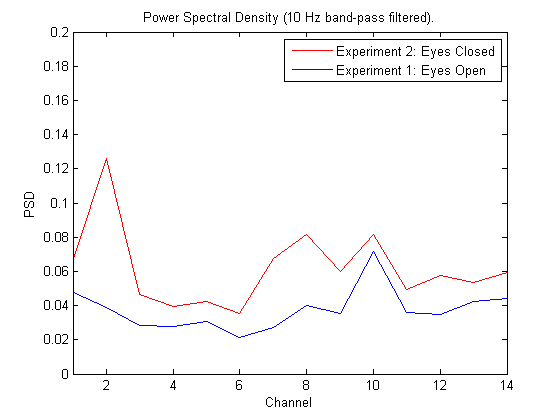
\includegraphics[scale=0.4]{PSDExperiment1VsExperiment2.png}
%      \caption{Power Spectral Density band-passed at 8-12 Hz, for each channel.  The two experiments shows different levels and it can be seen how the experiment 2 for the Drowsiness Dataset has always higher values.  Channels are numbered according to the device numbering system which corresponds to specific electrodes of the 10-20 international system\cite{c6,c11}. }
%      \label{psd}
%   \end{figure}
   
%Alpha Waves are 10 Hz signals, physiologically consistent across subjects, and they are associated with synchronous inhibitory processes and attention shifting \cite{c3}. They tend to be more prominent while the eyes are closed and appear stronger in occipital regions ($O_1$ and $O_2$ according to the 10-20 system \cite{c6,c11}). As can be seen in Fig. \ref{psd}, if we process the Drowsiness dataset with a 8-12Hz band-pass filter and calculate the average power spectral density across subjects and for each channel, we can see how clearly the value corresponding to class 2 (eyes closed) is always higher than the value for class 1 (eyes open), confirming the expected result.  This also verifies how the differentiation information is contained mostly in the frequency-domain.


\subsubsection{Dataset II - BCI Competition 2003 IIb \textit{self-paced 1s}}
We validated our method against the "BCI Competition 2003, dataset IV \textit{self-paced 1s}" \cite{c51}. This dataset is composed of 28 channels, in 416 epochs of 50 samples per epoch (500 ms length at 100 Hz) each one with the corresponding label, where subjects were asked to type at will a letter on a keyboard with the right or left index finger.  It is based on the Bereitschaftspotential \cite{c52}, which is a Slow Cortical Potential, particularly a slow change in voltages towards a negative potential drift, around 1000-500 ms before the onset of the self-initiated movement.  In this case, the information lies strongly on the time-domain.

%This dataset was recorded from a healthy subject during a no-feedback session. She/he sat in a normal chair with relaxed arms resting on the table and fingers in the standard typing position at the computer keyboard. The task was to press with the index and little fingers the corresponding keys in a self-chosen order and timing 'self-paced key typing'. The experiment consisted of 3 sessions of 6 minutes each. All sessions were conducted on the same day with some minutes break in-between. Typing was done at an average speed of 1 key per second.  


\subsection{Image Generation}

%The procedure must be independent of the experimentation protocol. COMO CUENTO ESTO GENERAL Y ESPECIFICO A LA VEZ.?

Data points are divided in non-overlapping rectangular window samples.  For each sampling window, we generate a binary image of a fixed height and width, which can be scaled by a factor $ \delta $.  The width is the size of the time interval of each window sample, and according to the sample rate of each dataset, it is 1280 data points for the Drowsiness dataset, and 50 for BCI Competition.  The height comes from the peak-to-peak amplitude according to the following equation:

$$
h(c) = |\max{   x(t,c) } - \min {x(t,c)}| \eqno{(2)}
$$ where $ x $ is the signal, $ t $ is time and $ c $ is the channel. Therefore, the height is calculated for each sample window and no clipping of the signal was performed. Additionally, the mean of the signal $ \bar{x}(c)  $ was subtracted from each window sample obtaining  $ \tilde{x}(t,c) = x(t,c) - \bar{x}(c)  $.  The image coordinate system assigns the point $ (1,1) $ to the upper left corner (increasing from top-to-bottom, from left-to-right). Hence, image $ I(z_1,z_2) $  values are:


$$
I(z_1,z_2) = \left\{ \begin{array}{rl}
255 & z_1 = \delta \cdot t, z_2 = \delta \cdot \tilde{x}(t,c) + \frac{h}{2} \\
0   & \mbox{otherwise}
\end{array}\right. \eqno{(3)}
$$ 
 

 
%\textit{The $ \delta $ is the aforementioned scale at which the image will be generated while $ h $ is the previously calculated height. As the only value which every pixel is effectively set is $ 255 $, the resulting image will be  mono-channel and binary.}

Finally, assigned pixels in the image were interpolated using the \textbf{Bresenham} \cite{c89} algorithm (see Fig. \ref{figure1} for an example).


   \begin{figure}[thpb]
      \centering
      \setlength\fboxsep{0pt}
	  \setlength\fboxrule{0.5pt}
      \fbox{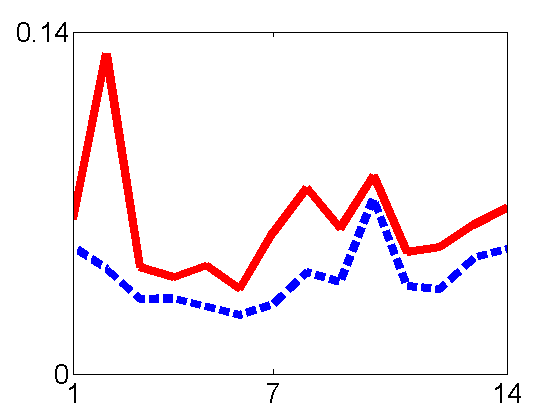
\includegraphics[width=2.5cm, height=1.8cm]{PSDExperiment1VsExperiment5.png}}
      \fbox{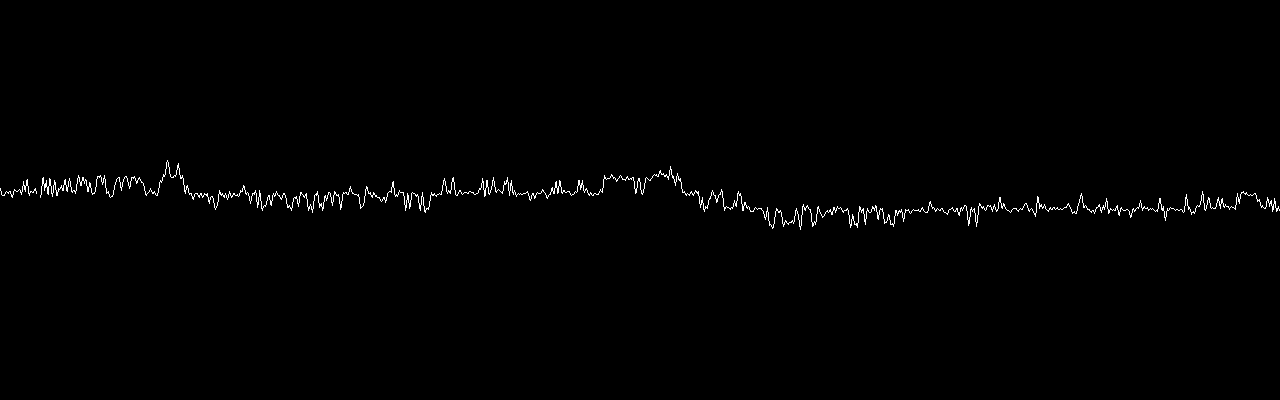
\includegraphics[width=2.5cm, height=1.8cm]{s_1_e_1_c_7.png}}
      \fbox{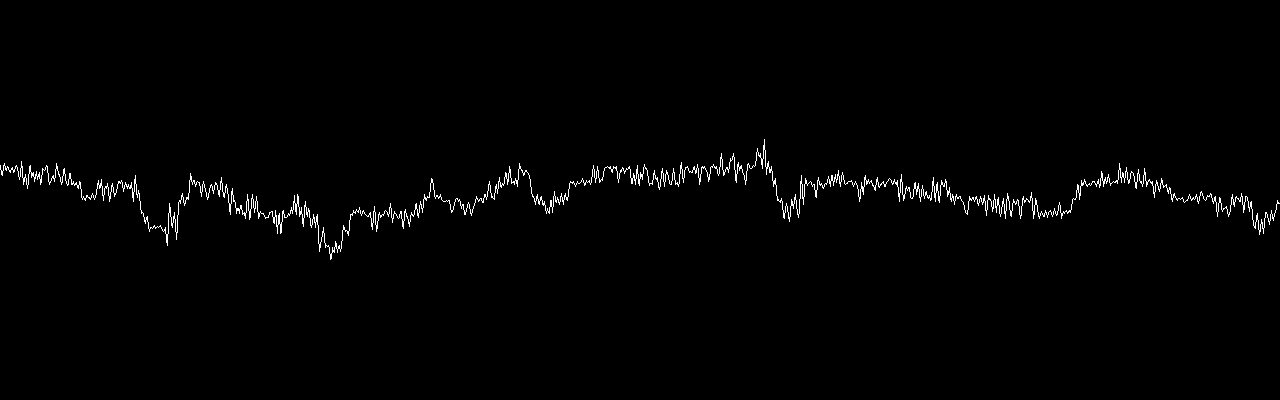
\includegraphics[width=2.5cm, height=1.8cm]{s_2_e_1_c_7.png}}
      \caption{PSD values for every channel (x-axis) are being shown for class 1, dashed line, and class 2, solid line, for Dataset I (left). EEG plot images corresponding to the subject 1 (center) and subject 2 (right) for the class 1 (eyes open), for the channel 7 ($ O_1 $) }
      \label{figure1}
   \end{figure}

   
\subsection{Feature Extraction: SIFT Descriptors} 




%In order to derive information from an image, with the purpose of Instance or Category Recognition, it is common to divide the task in keypoint detection and feature matching.  Keypoint detection relays on the extraction of salient intrinsic characteristics features and its description in a compact and stable (i.e. affine invariant) descriptive vector.  These  \textit{Descriptors} can be fed into a matching procedure, where a chained sequence of algorithms end up classifying each original image. 

The Scale-Invariant Transform Features (SIFT)\cite{c14} is a feature detection and classification method for images based on the extraction of salient intrinsic characteristics image keypoints, i.e. affine invariant image regions, and its characterization into a 128-dimensional  \textit{Descriptor} vector.  Using SIFT, different regions of different images can be compared and if the distance between the vectors is bellow a certain threshold, it represents some level of similarity (Fig. \ref{figure3}).  

%idea that certain characteristics, invariant to affine transformations,  could be detected by the difference of the convolution of Gaussian Kernels at different scales and orientations

%In Fig. \ref{figure3}, it can be seen how a descriptor around a keypoint shares visual similarity with another descriptor from a different image. 

%\textbf{Opcion II} In order to calculate identifiable features which are intrinsic characteristics that highlight specific data that help us to determine the kind of information that we are able to see from a given set (human beings still outperform machines in this task, so we are very used to use our own identification scale while measuring computer vision's systems performance).  The standard algorithm is divided in a first stage of "Feature Detection" following by a "Feature Description" and finally a bifurcation between "Feature Matching" and "Feature Tracking" being the former used to perform Category Recognition and the latter to implement Visual Tracking on streams of images (i.e. video). 

%\textit{SIFT features are detected by identifying local extrema, points or regions with salient features, using difference of Gaussian functions. Once they are detected, descriptors are obtained by computing the gradient at each pixel in a 16 x 16 image frame around the detected feature point.  In each 4 x 4 quadrant of the frame, a gradient orientation histogram is formed by adding weighted gradient value to one of the eight orientations ( $ \frac{pi}{8} $ ) histogram bins, which can be done by projecting the gradient onto the 8 orientations, but only considering the positive projected values.   The resulting 128 (8 orientations x 16 cells) non-negative values from a raw version of the SIFT descriptor vector.}

   
      \begin{figure}[thpb]
      \centering
      \setlength\fboxsep{0pt}
	  \setlength\fboxrule{0.5pt}
      \fbox{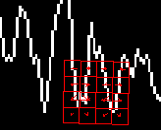
\includegraphics[scale=0.8]{s8e1c7d18.png}}
      \fbox{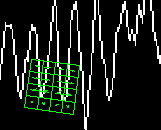
\includegraphics[scale=0.8]{s9e1c7d4.png}}
      \caption{A region around a keypoint in the left image was matched against a corresponding and visually similar region on the right image. These images correspond to the Drowsiness Dataset, channel 7 ($ O_1 $) for the class 1 (eyes open) for two different subjects.}
      \label{figure3}
   \end{figure}
   
     
\subsection{Matching Strategy}   

%\textit{The popular standard SIFT matching algorithm \cite{c14,c6} is regularly used to perform matching between descriptors in tandem with SIFT procedure.  However two characteristics of this algorithm were not appropriate for our approach.  The first one is that the algorithm is not commutative among the comparison operands which leads to different results depending on the their order.  The second is that the Nearest Neighbour Distance Ratio performed by the algorithm excludes specifically those matchings between a descriptor from one image against a set of similar descriptors from the second image.}

The procedure is detailed in Alg. \ref{algorithm1} and it works in a channel by channel basis.  In the first part, the set of descriptors  $ \mathcal{D} I(c,s) $ per channel $ c $ is obtained from the image $I(c,s)$, subject or epoch $ s $ for both classes.  In order to properly give more weight to edges in the binary image, the SIFT parameter edge-threshold $\epsilon$ was modified to reduce the sensibility of the threshold filter which is applied in the proposed algorithm \cite{c14}. The set of descriptors $ D(c) $ per channel are clustered using \textbf{k-medoids} \cite{c20} into $ F $ clusters.  This algorithm assigns as cluster center an original descriptor from $ D(c) $, not an interpolated one. The set of $ F $ descriptors is then stored into $ kmD(c) $ and each one will be considered as a \textit{visual feature}. The next step is to identify which ones are actually present on each image.  In order to perform this operation, the original descriptors are classified around the k-medoids centers using the nearest neighbour algorithm, i.e. \textbf{k-nn} \cite{c9}.   Finally, for every channel $ c $ and feature $ f $, binary feature vectors $O_i(c,f)$ for the whole set of images from both classes $(i=1,2)$, are created based on the clustering of the descriptors around features.  If a particular descriptor from any image of the same class is assigned to cluster $ f $ for the channel $ c $  then $ O_i(c,f) $ is set to 1, and 0 otherwise. The entire code was implemented in  \textsc{Matlab} (Mathworks, Natick, MA), and we used the \textsc{VLFeat} library \cite{c16} for SIFT processing.

%Those descriptors from both classes that have a higher number of matches against descriptors from other images from the same class, are filtered out (into $ D(c) $). In order to determine the matches, the \textbf{siftmatches} algorithm was used \cite{c16,c14,c9}. 


\begin{algorithm}
 \KwData{ Image per Sample Window $I(c,s)$ }
 \KwResult{ Discrimination Matrices $O_1$ and $O_2$ }
 \For{each epoch or subject \textbf{s}}{
	 \For{each channel \textbf{c}}{
	  $\mathcal{D}$I(c,s) $\leftarrow$ SIFT($I(c,s)$)\;
	  Add $\mathcal{D}$I(c,s) $\rightarrow$ D(c)\;
  	 }
 }
	  
 \While{per each channel}{
  kmD(c) $\leftarrow$ kMedoids(D(c))\;
 }
 \For{each epoch or subject \textbf{s}}{
	 \For{each channel \textbf{c}}{
	  \For{each descriptor \textbf{d} in $\mathcal{D}$I(c,s)}{
		$ f $ $\leftarrow$ \textbf{knn}( $d$, kmD(c)) \;
		$O_1(c,f)$	$\leftarrow$ $1$ when class is $1$\; 
		$O_2(c,f)$	$\leftarrow$ $1$ when class is $2$\;  
	  }
  	 }
 }
 \caption{Construction of Discrimination Matrices}
 \label{algorithm1}
\end{algorithm}
   
\subsection{Feature Translation}   

The elements from  $O_1(c,f)$ and $O_2(c,f)$ that are equal to zero, determine that none of the images from that class contains the feature $f$ for some specific channel $c$.  The set of tuples $ (c,f) $ can be used to classify to which set each image belongs, hence, to which class each sample window is classified.   This can be finally used as discrimination information, as long as $O_1(c,f) \neq O_2(c,f)$

\section{Results}

Results can be summarized in the Table \ref{table3}. Confusion Matrices for both datasets show that every sampled window was matched to its proper class, and no mismatch was found. 

\begin{table}[h]
        \footnotesize  \onehalfspacing
        \caption{Confusion Matrices for Dataset I (left) and Dataset II (right)}
		\begin{center}		
		\begin{tabular}{ c c }
		$\left[
		\begin{array}{c c}
		10 & 0 \\
		0 & 10 \end{array}
		\right] 
		$ & 
		$ \left[
		\begin{array}{c c}
		159 & 0 \\
		0 & 157 \end{array}
		\right]
		$ 
		\end{tabular}
		\end{center}
        \label{table3}
\end{table}

%Parameters for both the Feature Extraction and the Matching Strategy can be found on Table \ref{table2}.  The scale that was used to generate the image plot is represented by $ \delta $ and the edge-threshold \textbf{$\epsilon$} controls the sensitivity of the SIFT algorithm to filter borders.  The remaining is the Feature Vector Dimension $ F $ which controls the number of k-medoids cluster centers. We used the value $ k = 1 $ for the number of neighbours to consider on the \textbf{knn} algorithm.

Parameters for both the Feature Extraction and the Matching Strategy can be found on Table \ref{table2}: the scale $ \delta $ that was used to generate the image plot, the edge-threshold \textbf{$\epsilon$} which controls the sensitivity of the SIFT algorithm to filter borders and the Feature Vector Dimension $ F $ which controls the number of k-medoids cluster centers. We used $ k = 1 $ for the number of neighbours to consider on the \textbf{knn} algorithm.


\begin{table}[h]
        \footnotesize  \onehalfspacing
        \caption{Parameters values}
        \begin{tabular}{p{1.80cm}p{1.80cm}p{1.80cm}p{1.80cm}}
                \hline
                Dataset & $\delta$ & $\epsilon$ & F \\
                \hline
                I  & 1 & 10 & 200 \\
                II & 2 & 40 & 700 \\ 
                II & 4 & 15 & 700 \\               
                II & 8 & 10 & 700 \\
                \hline
        \end{tabular}
        \label{table2}
\end{table}


The selection of these parameters was performed empirically based on the following guidelines:  in order to obtain an adequate number of descriptors from SIFT, the edge-threshold $\epsilon$ was adjusted accordingly (i.e. greater than the default value of $ 10 $). This was due to the fact that a binary image is basically a contour image, and the sift edge response filtering should be loosen \cite{c14}.  At the same time, having too many descriptors is in detriment of the algorithm in terms of processing time and memory, thus its number must be bounded.  Lastly, the number of features $ F $ was increased accordingly until perfect classification was achieved.  A value slightly less than the one specified for $F$ is unable to classify images with low information content.

\section{Conclusion}

We presented a method for EEG signal feature extraction and classification.  We verified here that the procedure can be successfully applied to two physiologically meaningful datasets and that it is possible to discriminate known EEG signals based solely on their plots according to the proposed algorithm.

SIFT descriptors are easy and fast to calculate and they can be used to implement real-time operation.  Once a set of relevant descriptors can be found off-line for a given cognitive pattern, they can be used on single trial on-line procedures implementing protocols to transmit volition or any other control signal.  Additionally, the compact form of SIFT descriptors is also very useful as a characterization mechanism of EEG signals for regular BCI Feature Extraction and Classification steps \cite{c6}. 

\subsection{Future Work}

We used a direct image generation algorithm but other approaches can be selected to verify if better results regarding generalization performance can be obtained.  Additionally, empirical work on SIFT parameters and its usage on EEG images should be encouraged.  We found that the sensibility of the parameter selection is very high.  Extension to other BCI mental paradigms like P300, SSVEP, Visual Spatial Covert Attention, ErrP \cite{c6} and other similar phenomena, as well as, passive mental states, like alertness, will be desirable.  Furthermore, the extensive body of research on SIFT provides a fruitful path to explore in order to achieve faster and improved algorithms to automatically detect EEG characteristics which are suitable for classification. Other image processing feature extraction methods like SURF, GLOH, RANSAC could also be considered \cite{c9}.

\section*{Conflict of Interest}
The authors declare that they have no conflict of interest.


\section*{Acknowledgements}

%This project was supported by the ITBACyT-15 funding program issued by ITBA University.
This project was supported by NNNNN funding program issued by NNNNN.

\bigskip

\bibliography{paper}

%\begin{table}[h]
%\footnotesize
%        \begin{tabular}{ll}
%        &Author: R.Ramele \\
%        &Institute: Instituto Tecnológico de Buenos Aires \\
%        &Street: 25 de Mayor 457, 6th floor\\
%        &City: Ciudad de Buenos Aires \\
%        &Country:  Argentina \\
%        &Email: rramele@itba.edu.ar \\
%        \end{tabular}
%\end{table}

%\begin{table}[h]
%\footnotesize
%        \begin{tabular}{ll}
%        &Author: \\
%        &Institute: \\
%        &Street: \\
%        &City: \\
%        &Country:  \\
%        &Email: \\
%        \end{tabular}
%\end{table}


\end{document}
